\documentclass[aspectratio=169]{beamer}

\usepackage{beamerthemesplit}
\usepackage{amsmath}
\usepackage{amsfonts}
\usepackage{amssymb}
\usepackage{cancel}
\usepackage{bussproofs}
\usepackage{graphicx}

% For ⩘ and ⩗ (requires the LuaLaTeX engine)
\usepackage{unicode-math}
\setmathfont{Stix Two Math}

% For highlighting MeTTa code
\usepackage{listings}
\usepackage{color}
\definecolor{mygreen}{rgb}{0,0.6,0}
\definecolor{mygray}{rgb}{0.5,0.5,0.5}
\definecolor{mymauve}{rgb}{0.58,0,0.82}
\lstset{ %
  backgroundcolor=\color{white},   % choose the background color
  basicstyle=\tiny,                % size of fonts used for the code
  breaklines=true,                 % automatic line breaking only at whitespace
  captionpos=b,                    % sets the caption-position to bottom
  commentstyle=\color{mygreen},    % comment style
  escapeinside={\%*}{*)},          % if you want to add LaTeX within your code
  keywordstyle=\color{blue},       % keyword style
  stringstyle=\color{mymauve},     % string literal style
}

% Commands for Atomese code
\newcommand{\SP}{\;\;\;}
\newcommand{\TTrue}{\textit{True}}
\newcommand{\TFalse}{\textit{False}}
\newcommand{\TAtom}{\textit{Atom}}
\newcommand{\TTime}{\textit{Time}}
\newcommand{\TEval}{\textit{Evaluation}}
\newcommand{\TList}{\textit{List}}
\newcommand{\TLamb}{\textit{Lambda}}
\newcommand{\TExec}{\textit{Execution}}
\newcommand{\TAtTime}{\textit{AtTime}}
\newcommand{\TAnd}{\textit{And}}
\newcommand{\TOr}{\textit{Or}}
\newcommand{\TNot}{\textit{Not}}
\newcommand{\TImpl}{\textit{Implication}}
\newcommand{\TPredImpl}{\textit{PredictiveImplication}}
\newcommand{\TSeqAnd}{\textit{SequentialAnd}}
\newcommand{\TSeqOr}{\textit{SequentialOr}}
\newcommand{\TBSeqAnd}{\textit{BackSequentialAnd}}
\newcommand{\TFSeqAnd}{\textit{ForeSequentialAnd}}
\newcommand{\TLag}{\textit{Lag}}
\newcommand{\TLead}{\textit{Lead}}
\newcommand{\TTV}{\textit{TV}}
\newcommand{\TTVo}{\textit{TV}_1}
\newcommand{\TTVi}{\textit{TV}_i}
\newcommand{\TTVn}{\textit{TV}_n}
\newcommand{\TTVPo}{\textit{TV}_1^P}
\newcommand{\TTVQo}{\textit{TV}_1^Q}
\newcommand{\TTVPi}{\textit{TV}_i^P}
\newcommand{\TTVQi}{\textit{TV}_i^Q}
\newcommand{\TTVPn}{\textit{TV}_n^P}
\newcommand{\TTVQn}{\textit{TV}_n^Q}
\newcommand{\TTVP}{\textit{TV}^P}
\newcommand{\TTVQ}{\textit{TV}^Q}
\newcommand{\TTVR}{\textit{TV}^R}
\newcommand{\TTVPQ}{\textit{TV}^{PQ}}
\newcommand{\TTVQR}{\textit{TV}^{QR}}
\newcommand{\TBTV}{\langle \TTV \rangle}
\newcommand{\TBTVPo}{\langle \TTVPo \rangle}
\newcommand{\TBTVQo}{\langle \TTVQo \rangle}
\newcommand{\TBTVPi}{\langle \TTVPi \rangle}
\newcommand{\TBTVQn}{\langle \TTVQn \rangle}
\newcommand{\TBTVPn}{\langle \TTVPn \rangle}
\newcommand{\TBTVQi}{\langle \TTVQi \rangle}
\newcommand{\TBTVP}{\langle \TTVP \rangle}
\newcommand{\TBTVQ}{\langle \TTVQ \rangle}
\newcommand{\TBTVR}{\langle \TTVR \rangle}
\newcommand{\TBTVPQ}{\langle \TTVPQ \rangle}
\newcommand{\TBTVQR}{\langle \TTVQR \rangle}
\newcommand{\Tstrength}{\textit s}
\newcommand{\Tconf}{\textit c}

% Commands for symbolic mathematical notations
\newcommand{\prob}[1]{\mathcal{Pr}\left(#1\right)}
\newcommand{\mean}{\textit{mean}}
\newcommand{\cnt}{\textit{count}}
\newcommand{\poscnt}{\textit{pos\_count}}
\newcommand{\sat}[1]{\mathcal{S}(#1)}
\newcommand{\ltv}[1]{<\!\!#1\!\!>}
\newcommand{\letv}[2]{(#1, #2)}
\newcommand{\limp}{\rightarrow}
\newcommand{\lpreimp}[1]{\leadsto^{#1}}
\newcommand{\lseqor}[1]{\bigslopedvee^{#1}}
\newcommand{\lseqand}[1]{\bigslopedwedge^{#1}}
\newcommand{\lbseqor}[1]{\reflectbox{$\bigslopedvee$}^{#1}}
\newcommand{\lbseqand}[1]{\reflectbox{$\bigslopedwedge$}^{#1}}
\newcommand{\ldo}[1]{\widehat{#1}}
\newcommand{\llag}[2]{\overrightarrow{#1}^{#2}}
\newcommand{\llead}[2]{\overleftarrow{#1}^{#2}}

\makeatletter
\newcommand{\reallytiny}{\@setfontsize{\srcsize}{2pt}{2pt}}
\makeatother

\mode<presentation>
{
  \usetheme{AnnArbor}
  \usecolortheme{crane}
}

\usepackage[english]{babel}
%% \usepackage[latin1]{inputenc}
\usepackage{times}
\usepackage[T1]{fontenc}

\title{Rational OpenCog Controlled Agent}

\author{Nil Geisweiller, Hedra Yusuf}

\institute[SingularityNET OpenCog Foundations]
{
  \begin{center}
    AGI-23\\
    
\includegraphics[scale=0.32]{pictures/snet_oc.png}
  \end{center}
}

\date[AGI-23]

\begin{document}

\section{Introduction}

\begin{frame}
  \maketitle
\end{frame}

\begin{frame}

  \begin{center}
    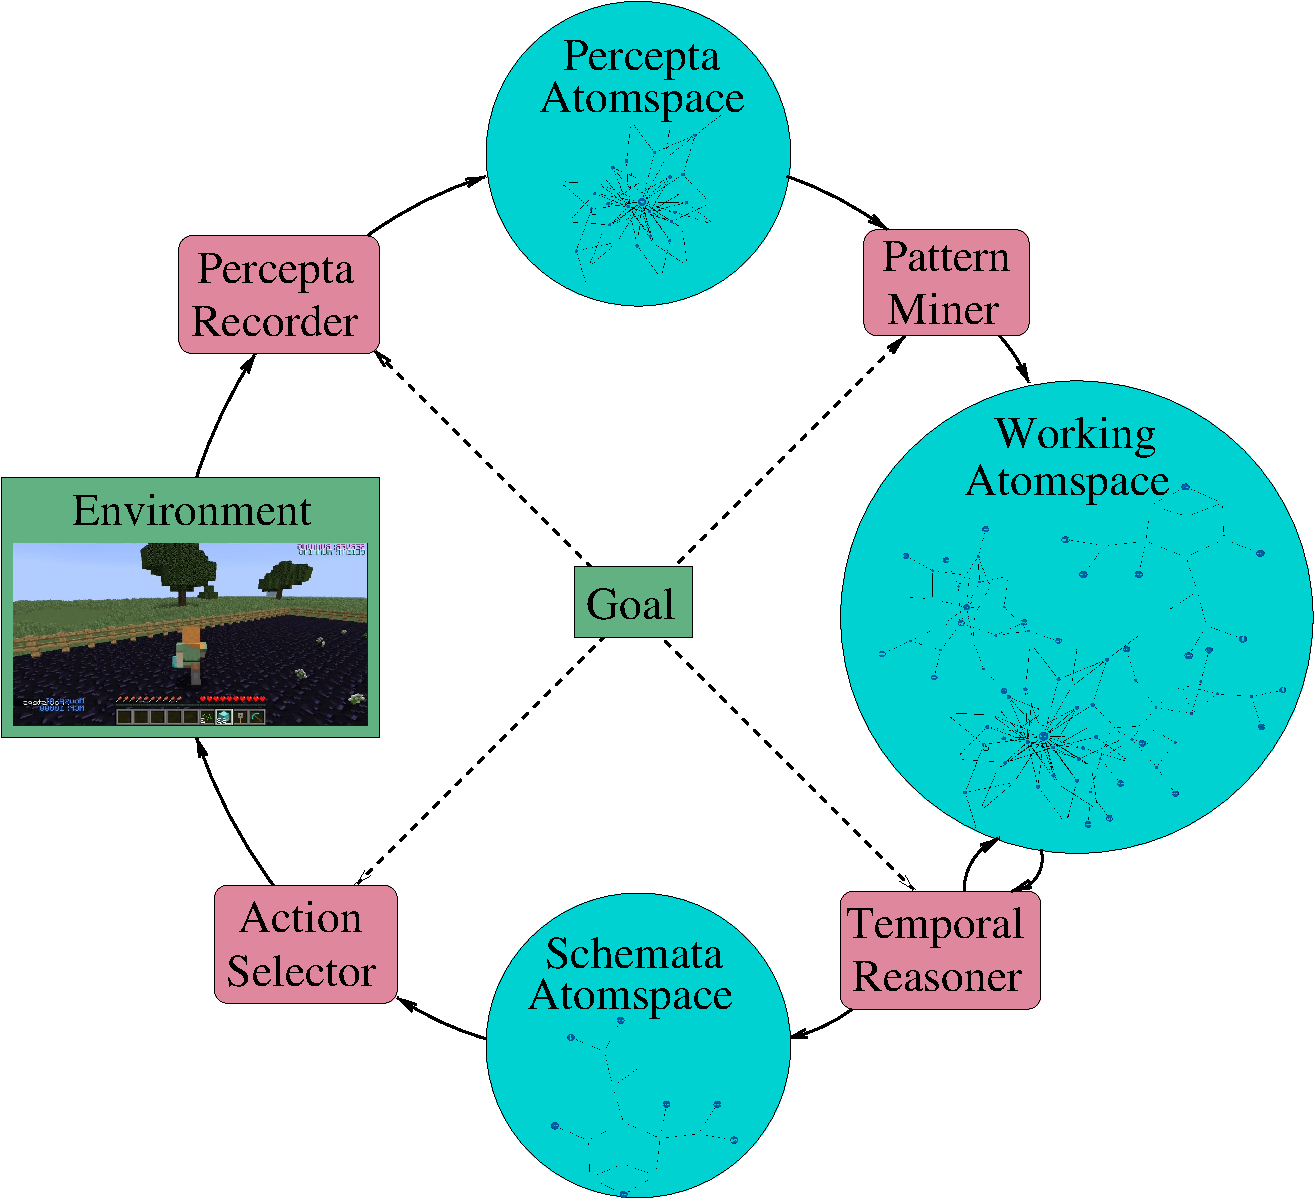
\includegraphics[width=0.54\textwidth]{pictures/rocca-chart-v0.7.pdf}
  \end{center}

\end{frame}

\section{Planning}

\begin{frame}

  % <BEGIN-SPEECH>
  % Everything that is turn to the past is left associative, everything
  % that is turned to the future is right associative, and that way we
  % can remove all parenthesis and read from the left to right, in
  % chronological order.
  % <END-SPEECH>

  \begin{center}
    \only<1>{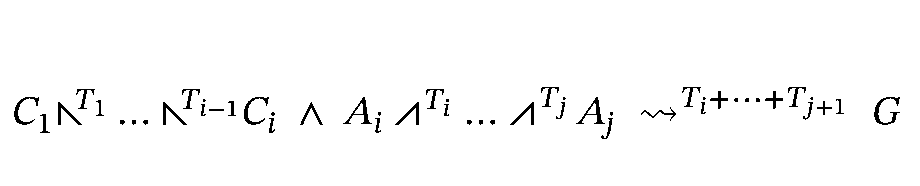
\includegraphics[scale=0.4]{pictures/schema-not-decorated.png}}
    \only<2->{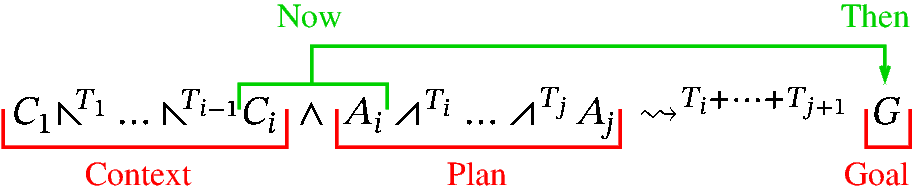
\includegraphics[scale=0.4]{pictures/schema-decorated.png}}
  \end{center}

  % <BEGIN-SPEECH>
  % Well, in a way everything is happening now, because, you remember I
  % said that this operator brings the past into the present, and that
  % one, and that one too, brings the future into the present, so
  % everything is from the viewpoint of the present.  But of course we
  % can't evaluate what is coming from the future, but everything else
  % we can.  So for instance if t is now, then we can evaluate
  % <END-SPEECH>

  \pause
  \pause

  {\large
    $$
    \begin{array}{ccc}
      \left[ C_1 \lbseqand{\!\! T_1} \dots \lbseqand{\!\! T_{i-1}} C_i
      \right](t) & = & \textit{True}\ |\ \textit{False}\\
      \pause & \mapsto & \mathcal{Dist}(Bool) \\
      \pause & \mapsto & \mathcal{Dist}(\mathcal{Dist}(Bool)) \\
    \end{array}
    $$
  }

  % <BEGIN-SPEECH>
  % And normally we should be able to evaluate to True or False, unless of
  % course the predicates are inherently uncertain, or we have forgotten
  % the past, etc, in which case it will be evaluated to a Bernouilli distribution,
  % possibly even a second order Bernouilli distribution.
  % <END-SPEECH>

\end{frame}

\begin{frame}
  \frametitle{It is always now}

  % <BEGIN-SPEECH>
  % So for instance if all you've got is this schema, then in order to
  % continue the plan after taking the first action, you need to at
  % least apply temporal transposition so that the follow-up of the
  % plan is expressed from the view point of now.
  %
  % So that after selecting action A1, then A2 becomes the present
  % action, and A1 becomes the context, and then A3 becomes the
  % present action and A2 becomes the context as well.  And of course
  % you're getting closer and closer to the goal.
  % <END-SPEECH>

  {\huge
    $$
    C \land A_1 \lseqand{T_1} A_2 \lseqand{T_2} A_3
    \lpreimp{T_1+T_2+T_3} G
    $$
    $$
    C \land A_1 \lbseqand{\!\! T_1}\ A_2 \lseqand{T_2} A_3 \lpreimp{T_2+T_3}
    G
    $$
    $$
    C \land A_1 \lbseqand{\!\! T_1} A_2 \lbseqand{\!\! T_2}\ A_3 \lpreimp{T_3} G
    $$
    }
\end{frame}

\begin{frame}
  \frametitle{Example of schemata}

  Collect diamonds
\end{frame}

\begin{frame}
  \frametitle{Learning schemata}
\end{frame}

\begin{frame}
  \frametitle{Balancing exploitation and exploration}
\end{frame}

\end{document}
